\section{Stage 2: \jpc{}, pathwise RL with a jointly trained critic}
\label{sec:method}
Stage 1 left the chain's defining property unused: every transition of~(\ref{eq:chain}) is differentiable. If a critic $V_\phi(y_k)\approx\mathbb E[r\mid y_k,c]$ can score a noisy intermediate state, then reparameterising one transition, $y_k=\alpha_kD_\theta(y_{k-1})+\sigma_k\varepsilon_k$, gives the pathwise estimator
\begin{equation}
\hat g_{\mathrm{PW}}=\sum_{i\in\mathcal G}\frac{\partial V_\phi(y_k)}{\partial y_{k,i}}\,\alpha_k\,\frac{\partial D_\theta(y_{k-1})_i}{\partial\theta},
\label{eq:pw}
\end{equation}
an unbiased estimate of that transition's share of $\nabla_\theta J$ when the critic is exact (Appendix~\ref{app:pw_derivation}). Where the score~(\ref{eq:sf}) multiplies the injected noise, (\ref{eq:pw}) sends each coordinate a deterministic signal, the critic's local slope, which vanishes on coordinates the outcome does not depend on. Everything therefore rests on the critic. This section builds it in two steps, first over the flow-step axis and then over both axes of the chain, and then gives the training procedure; Algorithm~\ref{alg:jpc} is complete enough to implement either critic from.

\paragraph{Two axes of credit.}
In an AR model the RL time step is the token position, so actions, advantages and values are all indexed by position: credit is one-dimensional. A flow model generates every position at once and refines it over $K$ steps, so a generation is a $K\times L$ grid of states $y_{k,i}$ (\S\ref{sec:estimators}), and a token is decided gradually, along the flow, at its position. Ports of RL to flow models keep one axis, the flow step, and treat the whole $L\times d$ state as the action \citep{liu2025flowgrpo,xue2025dancegrpo}; that is the estimator of \S\ref{sec:grpo}. A critic for a flow language model should be indexed by both: \emph{when} along the flow ($k$) and \emph{where} along the sequence ($i$).

\paragraph{Step 1: a scalar critic over flow steps.}
Treat the flow step as the time step of an MDP with state $y_k$ and a single terminal reward $r$. Its value $V(y_k)=\mathbb E[r\mid y_k,c]$ is defined at every step and needs no per-step labels: roll out the sampler, keep the outcome and a few intermediate states, and fit $V_\phi$ by binary cross-entropy of $\sigma(V_\phi(y_k))$ against $r$. The critic reuses the denoiser: a copy of $D_\theta$'s transformer gives per-position features $f_i(y_k,t_k,c)$, which are averaged over the generated positions $\mathcal G$ and passed to a small head, $V_\phi(y_k)=h_\phi\big(\tfrac1{|\mathcal G|}\sum_{i\in\mathcal G}f_i,\,t_k\big)$. Ascending this critic with~(\ref{eq:pw}) already works, but it is fragile (\S\ref{sec:experiments}): the gradient reaches position $i$ only through the pooled feature, so an undecided position and a committed one receive the same instruction.

\paragraph{Step 2: the 2D critic.}
Give every position its own value and pool afterwards:
\begin{equation}
R_{k,i}=h_\phi\big(f_i(y_k,t_k,c),\,t_k\big),\qquad V_\phi(y_k)=\frac1{|\mathcal G|}\sum_{i\in\mathcal G}R_{k,i}.
\label{eq:critic2d}
\end{equation}
The critic is now a field over flow steps and token positions; the actor still ascends the pooled value, but $\partial V_\phi/\partial y_{k,i}$ now passes through position $i$'s own head, so every position of the state receives its own signal. The scalar critic is the pool-then-head special case. The field is supervised twice: through its mean, by the outcome, and position by position, by the same outcome (each $R_{k,i}$ is asked to predict $r$), which keeps the per-position values informative during training.

\paragraph{Training the critic with the policy.}
A critic trained once on the base policy is exploited within a few hundred updates: its value keeps rising while the true success rate falls (\S\ref{sec:ablations}). \jpc{} therefore trains the critic on the policy's own rollouts throughout. Each iteration rolls out $B$ prompts under the deployment sampler and stores the states of every trajectory at five evenly spaced steps of the RL window, with their outcomes, in a replay buffer; the actor takes one pathwise step~(\ref{eq:pw}) at a random step of the window; the critic then takes two gradient steps on the buffer. The states the critic learns from are thus drawn from the same window and the same policy as the states at which the actor queries it. Two safeguards keep the critic ahead of the actor: every ten iterations the critic's pooled value is scored against the outcomes of the newest buffer states, and if its discrimination (AUC) at any stored step drops below $0.9$ the critic takes eight extra steps; and the actor's learning rate decays on a cosine from $10^{-6}$ to $10^{-7}$, which removes the late collapse that a constant rate produces. Before RL the critic is pre-trained on rollouts of the base policy (Appendix~\ref{app:details}); its quality is the one task-dependent lever we found, and it is decisive (\S\ref{sec:ablations}).

\paragraph{Sampler and stopping rule.}
Gains lock to the sampler they were trained under (\S\ref{sec:ablations}), so training uses the sampler that will be deployed; \S\ref{sec:loop} later carries the gains to cheaper samplers. Checkpoints are evaluated on held-out prompts and the peak is reported, since on Game24 the training success rate is not a proxy for held-out accuracy.

\begin{algorithm}[t]
\caption{\jpc{}: pathwise RL with a jointly trained critic (scalar or 2D)}
\label{alg:jpc}
\small
\begin{algorithmic}[1]
\REQUIRE policy $D_\theta$ (task-SFT model); verifier $r$; deployment sampler $(\gamma,K)$ giving the chain~(\ref{eq:chain}); RL window $[k_{\mathrm{lo}},k_{\mathrm{hi}}]$ ($[8,40]$ of 64; $[4,20]$ of 32); critic $\phi$ = trunk $f$ (copy of $D_\theta$) + head $h_\phi$, with $V_\phi(y_k)=h_\phi(\mathrm{mean}_{i\in\mathcal G}f_i,t_k)$ (\textbf{scalar}) or $V_\phi(y_k)=\mathrm{mean}_{i\in\mathcal G}\,h_\phi(f_i,t_k)$ (\textbf{2D}, eq.~\ref{eq:critic2d}); prompts per iteration $B{=}32$; buffer capacity $N{=}16$k; critic steps $m{=}2$, extra steps $m'{=}8$, AUC floor $0.9$; actor learning rate $10^{-6}$ with cosine decay to $10^{-7}$; critic learning rate $10^{-5}$.
\STATE \textbf{Pre-train $\phi$:} roll out $D_\theta$ under the deployment sampler on 32k prompts; store $(y_k,t_k,c)$ at five evenly spaced steps and the outcome $r$; minimise $\mathrm{BCE}(\sigma(V_\phi(y_k)),r)$ for up to 12 epochs; keep the epoch with the best held-out AUC.
\FOR{iteration $=1,\dots,T$}
  \STATE Sample $B$ prompts; roll out the chain~(\ref{eq:chain}) for $K$ steps without gradients; decode; verify $r$.
  \STATE \textbf{Actor:} draw $k\sim\mathcal U\{k_{\mathrm{lo}},\dots,k_{\mathrm{hi}}\}$; recompute $y_k=\alpha_kD_\theta(y_{k-1})+\sigma_k\varepsilon_k$ with gradients through $D_\theta$; $\theta\leftarrow\theta+\eta_\theta\nabla_\theta V_\phi(y_k)$ (Adam, gradient clipped at 1).
  \STATE \textbf{Buffer:} from the same rollouts push $(y_k,t_k,c,r)$ at five evenly spaced $k$ in the window; keep the newest $N$.
  \STATE \textbf{Critic:} $m$ steps on buffer minibatches of 64 with loss $\mathrm{BCE}(\sigma(V_\phi),r)$; for the 2D critic average it with $\tfrac1{|\mathcal G|}\sum_i\mathrm{BCE}(\sigma(R_{k,i}),r)$.
  \STATE Every 10 iterations: AUC of $V_\phi$ against $r$ on the newest 256 buffer states at each stored $k$; if the minimum is below $0.9$, take $m'$ extra critic steps.
  \STATE Every $S$ iterations: save $(\theta,\phi)$; evaluate $\theta$ on held-out prompts; report the peak.
\ENDFOR
\end{algorithmic}
\end{algorithm}

\begin{figure}[t]
\centering
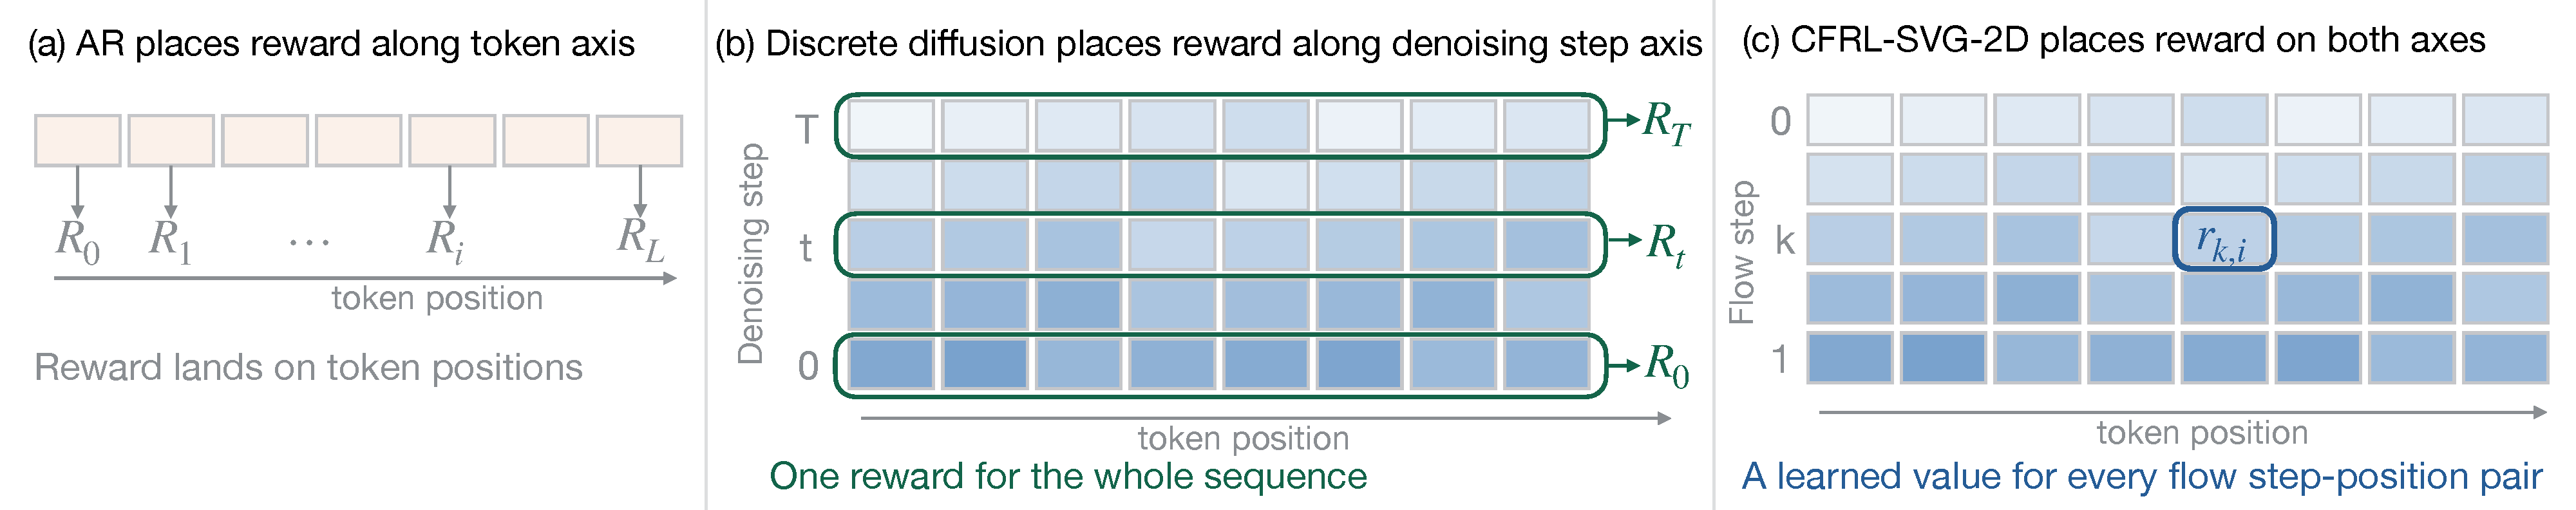
\includegraphics[width=0.78\linewidth]{figures/flow-rl-figure1.pdf}
\caption{(a) A reward bit attaches to $\sim$30 categorical decisions in an AR model but is spread over $10^{5}$--$10^{6}$ noise coordinates in a flow language model, whose score is the noise itself; the pathwise gradient replaces it with a deterministic per-coordinate signal from a critic on noisy states. (b) \jpc{}: the 2D critic scores every position $i$ of a random intermediate state $y_k$, its pooled value is the actor's objective, and it is trained on the same rollouts as the policy.}
\label{fig:mechanism}
\end{figure}
